% !TEX root = ../main.tex
% !TEX program = XeLaTeX
% !TEX encoding = UTF-8 Unicode

\date{2018년 3월 21일}

\begin{frontmatter}
\title{축치어}
\author{양재영}
\address{서울대학교}
\begin{abstract}
Dunn, Michael. (1999). A Grammar of Chukchi. PhD dissertation, Australian National University, 61--118.
\end{abstract}
\end{frontmatter}

%%%%%

\section*{발제 범위 분배}
\begin{table}[h]
\begin{center}
\def\arraystretch{1.5}
\begin{tabular}{>{\sffamily}ccccl}
\hline
	&\itshape 발제자	&\itshape 발제 범위		
	&\itshape 페이지	&\itshape 내용\\
\hline
1	&김민규	&Ch. 1--3	&pp. 1--60		&서론, 방언, 음운론 \& 형태음운론\\
2	&양재영	&Ch. 4--6	&pp. 61--118	&품사, 문장, 명사류 굴절\\
3	&		&Ch. 7--9	&pp. 119--174	&대명사, 명사류 파생, 복합 명사류\\
4	&		&Ch. 10--11	&pp. 175--220	&동사 굴절, 결합가\\
5	&		&Ch. 12--13	&pp. 221--252	&동사 포합, 비정형 동사파생 형태\\
6	&		&Ch. 14--15	&pp. 253--290	&동사 파생, 장소적 관계\\
7	&		&Ch. 16--17	&pp. 291--324	&형용사 \& 수사, 계사 \& 보조사\\
8	&		&Ch. 18--19	&pp. 325--360	&부정문, 화용론\\
\hline
\end{tabular}
\end{center}
\label{default}
\end{table}

%%%%%
\setcounter{section}{3}
\section{품사}
\subsection{서론}
단어는 거의 항상 모음조화의 단위와 일치하며, 어간(과 해당하는 품사의 고유 굴절)로 구성된다. 음운론적 단어와 통사론적 단어를 구별할 필요는 없다. 하나의 어간이 서로 다른 품사로 통용되는 경우도 있다. 예컨대 \textbf{rˀe\textsuperscript{-VH}} `무언가(를 하다)' $\rightarrow$ \textbf{ɣa>rˀa<ma} `무언가를 가지고(ASSOC)/무언가를 하면서’
\subsection{명사류}
SAO 논항 관계, 계사의 보어, 공간 관계를 나타내는 격, 비복수/복수, 보통 절대격에서만 표시되는 인칭의 세 범주에 따라 굴절한다. 비복수가 무표적 수이고, 복수화는 언제나 가능하다. 대명사 또는 고등생물명사의 경우를 제외하고 엄밀한 단수를 의미하는 개별화가 가능하다.
\subsubsection{명사}
격은 항상 표시된다. 일반명사의 절대격이나 고등생물명사의 (등격 제외) 모든 격에서 수와 인칭이 표시된다. 고등생물명사는 인명을 포함하며, 친족 호칭 및 고등 생물을 지칭하는 지시사의 경우 유동적으로 포함한다. 고등생물명사는 능격/구격, 처격, 여격/향격 표지를 삭제시키는 단수 표지 \textbf{-ne\textsuperscript{-VH}}가 존재한다.
\subsubsection{대명사}
\begin{enumerate}
	\item 인칭대명사: 고유한 인칭과 수를 가지며, 때로는 지소나 확대 등의 파생이 일어난다.
	\begin{center}
	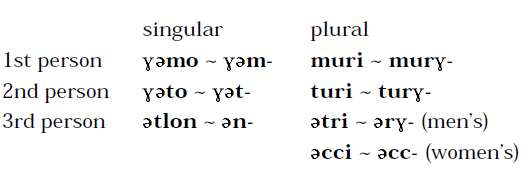
\includegraphics{Chukchi/src/chpr.png}
	\end{center}
	\item 부정/의문대명사: 인칭대명사와 동일한 특징
	\begin{center}
	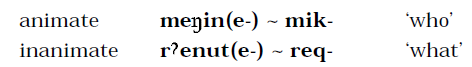
\includegraphics{Chukchi/src/chin.png}
	\end{center}
	\item 양화대명사: \textbf{əməlˀo} `모두’, \textbf{qut-} (\textbf{qol} `(나머지)하나’\footnote{\textbf{ənnen} `1’과 교체 가능한 동격 수식어로도 기능하나, 수사와 달리 격을 받고 논항이 될 수 있다.}, \textbf{qutti} `일부/나머지’)
	\item 지시대명사: 단수에서는 보통명사처럼 곡용하는 경향이 있다.
	\end{enumerate}
\subsubsection{분사}
동사에서 파생된 명사이며, 때로는 논항을 취하기도 한다. 주로 자동사에서 형성되며 타동사의 경우 역수동태화 후 형성되는 경향이 강하다. 즉 결합가가 1인 동사에서 파생된다.
\subsection{형용사}
형용사 어간과 품사로서의 형용사를 구분할 필요가 있다. 전자는 형용사 단어의 어휘핵으로 기능하지만 다른 기능도 수행하며, 후자는 보편/습관상 술어 또는 절대격으로 쓰여 한정 기능을 한다. 한정성 어간은 종종 절대격 핵어에 다른 격으로 포합된다. 자유 형용사는 습관상 동사와 동일하게 인칭/수를 교차 지시하며, 다른 시제로 표현할 경우 분석적 동사의 부사 핵으로서 나타난다. 자유 형용사는 형태적으로 습관상 자동사와 동일하나, 다음과 같은 점에서 구별된다.
\begin{enumerate}
	\item 다른 TAM 범주를 표시하지 못한다.
	\item 파생 접사가 형용사화 접환사 바깥에 붙는다. 예컨대 지소사 \textbf{n-$\rule{1cm}{0.2mm}$-qine-qej} vs. \textbf{n-$\rule{1cm}{0.2mm}$-qeet-qin}.
	\end{enumerate}
\subsection{수사}
419까지 20진법 체계가 존재하나, 오늘날의 화자들은 잘 이해하지 못한다. 수사는 구조에 따라 다음의 세 가지로 나뉜다.
\begin{enumerate}
	\item 단일 수사 어간: 1--5, 10, 15, 20 (cf. 고전 나와틀어 20진법 체계)
	\item 합성어 수사: 6--9, 11--14, 16--19, 20의 배수
	\item 분석적 수사: 20의 배수 + 나머지 + \textbf{pacol} `추가'
\end{enumerate}
또한 의문사 \textbf{tˀer/tˀec} `얼마나/그만큼' 역시 수사와 동일한 형태를 보인다. 수사는 격을 표시하지 않으나 S/O 논항 역할을 할 수 있으며, 수식하는 방식은 형용사와 유사하다. 서수(\textbf{-qew}), 배수(\textbf{-ce}), 인간 집합(\textbf{-rɣire}), 비인간 집합(\textbf{-jono}), 분배(\textbf{-jut}) 등의 고유 파생 접사들이 존재한다. 
\subsection{굴절 동사}
굴절 동사는 핵심 참여자의 인칭과 수에 일치하고, 시상법에 따라 굴절한다. 형태에 따라 자동, 타동, 유동으로 나뉘며, 타동성은 동사의 일치 패턴으로 표시되지만 서로 다른 결합가가 동일한 패턴을 보이는 경우도 있다. 어근에 따라 다음의 여섯 가지 논항 구조 유형이 존재한다.
\begin{itemize}
	\item 자동
	\begin{enumerate}
		\item 0자리 (vi-): 대부분 S 논항이 포합된 자동사, 일부는 기상 현상
		\item 1자리 (vi): 전형적 자동사
		\item 2자리(이상) (vi+): 필수 사격 부가어가 존재(하거나 맥락상 추론할 수 있는) 자동사
	\end{enumerate}
	\item 타동
	\begin{enumerate}
	\setcounter{enumi}{3}
		\item 2자리 (vt): 전형적 타동사
		\item 3자리(이상) (vt+): 필수 부가어가 있는 타동사 (여러 하위 유형 존재)
	\end{enumerate}
\end{itemize}
\begin{enumerate}
\setcounter{enumi}{5}
	\item 유동 (vlab): 자동사도 타동사도 될 수 있으며 그에 따라서 표시된다. 자동사에서 타동사로의 영표지 파생으로 (혹은 그 반대로) 볼 수도 있다. 
\end{enumerate}
핵심 논항이 포합되면 결합가가 감소하지만, 비핵심 논항을 포합하는 경우는 그렇지 않다. 계사는 1--2자리 자동사이다.
\subsubsection{분석적 동사}
조동사와 굴절되지 않은 어휘핵으로 이루어져 있다. 보통 어휘핵은 동사 어기, 동사에서 패생된 부사형, 형용사 등이다. 예컨대 \textbf{ləɣi n-ine-lɣ-ə-qin}	know.Vbase HAB-TR-AUX-E-3sg.
\subsubsection{조동사 \& 계사}
조동사는 분석적 동사에서 시상법과 타동성을 표시한다. 계사와 많은 형태를 공유한다. 아래의 \textbf{it-}과 \textbf{nˀel-}은 자동사의 조동사로 사용된다.
\begin{center}
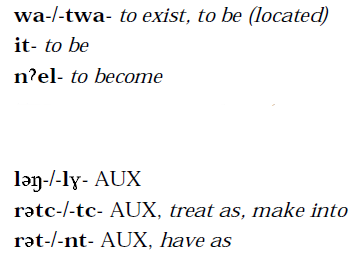
\includegraphics{Chukchi/src/chau.png}
\end{center}
타동사의 조동사 중 \textbf{rətc-/-tc-} 형태는 타동성 정신 활동(생각하다 등)에 귀결적인 의미를, \textbf{ləŋ-/-lɣ-} 형태는 비귀결적인 의미를 부여한다. \textbf{rət-/-nt-} 형태는 \textbf{-(t)e}로 끝나는 동사나 부정 동사 어기와 결합한다. \textbf{ləŋ-/-lɣ-}는 타동사 계사성 기능도 하며, 나머지 형태들은 주동사로도 쓰인다.
\subsection{동사 어기}
동사 어기는 분석적 동사의 어휘핵이나 부사로 기능한다. 붙을 수 있는 파생 접사는 다음과 같다.
\begin{center}
\begin{tabular}{llll}
극성	&접사	&결합 어근	&기능\\
\hline
긍정	&\textbf{-ɣtə}	&속성 동사	&자동사\\
	&\textbf{n><ˀew}	&\& 형용사	&어기 형성\\
	&\textbf{-u}	&정신 활동 동사	&타동사 어기 형성 (부사 기능 X)\\
	&\textbf{-(t)e}	&기타 동사	&(종종 다른 파생 접사 수반)\\
\hline
부정	&\textbf{e><ke}	&상적	&으로\\
	&\textbf{luŋ><(t)e}	&다	&름\\
\hline
\end{tabular}
\end{center}
파생되지 않은 동사 어기는 -u 파생 어기와 동일한 통사적, 의미적 성격을 띤다. 부정 존재 불변사 \textbf{ujŋe}와 방식 의문 부사 \textbf{miŋkəri} 등 일부 부사나 불변사도 파생되지 않은 동사 어기로 기능한다.
\subsection{부동사}
\textbf{-ma, -k, -ineŋu}가 동사에 붙어 부사절처럼 기능할 수 있게 한다. 부동사는 명사류 의존어를 가지기도 하나 그에 대해 일치는 표시되지 않는다. 각 접사는 특정 상이나 서법 관계를 결정하나, 체계적(paradigmatic)이지는 않다. \textbf{erɣatək} dawn-E-SEQ `내일' 에서처럼 문장 전반 수식 기능을 하기도 한다.
\subsection{부사 \& 불변화사}
인칭, 수, 격, 시제, 상, 서법에 따라 굴절하지 않는 닫힌 부류들로서 서로 무관하다. 여타 품사의 어간에서 파생된 경우 부사, 문법적 의미를 갖는 자립 형태소는 불변화사로 구분한다. 불변사에도 강의어나 제한/지소 접사를 통해 종종 파생이 일어난다.
\subsubsection{형용사 파생 부사}
형용사 어간에 접환사 \textbf{n><ˀew}를 붙여 만든다. 자동사 어기로도 기능한다. 비교급은 형용사 어간에 접미사 \textbf{-ŋ}를 붙여 만든다.
\subsubsection{지시 부사}
지시(대명사) 어간에 접사를 붙여 만드나, 패러다임 내에 빈자리나 불규칙형이 존재한다.
\subsubsection{파생되지 않은 시간 및 방식 부사}
대부분 시간적인 의미를 나타낸다. \textbf{tite} `언제?/언젠가'는 의문/부정의 기능을 모두 수행한다. `동사에서 파생된' 부사는 사실 부사 기능을 하는 부동사이다. 어미 \textbf{-ŋit}은 \textbf{lˀeleŋit} `겨울/겨울에/겨울을 나다'와 같이 부사, 명사, 동사로 기능하는 단어를 형성한다. 대부분의 방식 부사는 파생형이지만, 공동격성 관계를 표현하는 부사나 \textbf{iˀam} `왜'는 파생되지 않은 형태이다.
\subsubsection{명사구 수식 부사}
문장에서 절대격 명사류처럼 행동하며, 절대격 명사류로 대체 가능할 때도 있다. 양화사형 \textbf{cəmqək} `나머지', 재귀형 \textbf{cinit} `스스로', 제한형 여러 가지 등이 존재한다. 
\subsubsection{부정 소사}
\textbf{qərəm/qəcəm}과 \textbf{wanewan}은 의도법 동사와 쓰여 부정 술어를 만든다. \textbf{ənŋe}는 부정 부동사와 쓰여 금지 명령을 만든다. \textbf{ujŋe}는 (부정 부동사와 동음이의인) 결여격 명사류와 쓰인다. 부정 정체성 불변사 \textbf{qərəmena-/qəcəmena-}는 독립적인 품사 (하위)부류로서, 술어의 인칭/수와 일치를 표시하나 격은 표시하지 못하며, 일치하는 요소들과 함께 명사구를 형성하지 않는다.
\subsubsection{절 대치 소사}
명제 하나를 통째로 담고 있는 단어로, 감탄사 부류와 연속체를 이룬다. 판정의문문의 답변으로 쓰이는 부정 불변사도 이 범주에 속한다. \textbf{qoro} `다오'는 `주어진 것'에 해당하는 절대격의 통사적 종속어를 갖기도 하는 `타동절 대치 불변사'이며, \textbf{*qor} `여기로'와 동근일 가능성이 있다(Stebnickij 1994).
\subsubsection{접속 소사}
두 술어/절이나 명사류/명사구를 연결하는 기능을 한다. 술어/절 접속 불변사는 문장 전체를 이끌 수 있으며 인과관계 혹은 시간상의 연속 관계 등을 특정하기도 한다. \textbf{ənraq} `이/그때' 등은 절/문장을 시작하는 데 특화된 접속 소사이다.
\subsubsection{서법 소사}
미래 시제나 의도/조건법 동사와 쓰인다. \textbf{camˀam} ‘할 수 없다’, \textbf{mecənkə} ‘할 수 있다’의 경우 동사 보어 없이도 쓰일 수 있다.
\subsubsection{담화 소사}
증거성, 화자나 절 참여자들에 대한 행위의 감정적인 영향, 행위의 강도 등을 표현하는 다양한 불변화사가 여기에 속한다. 강조 담화 불변 접어 \textbf{=ˀm}은 흔히 쓰이며 어느 품사에든지 붙을 수 있다.
\subsubsection{평가 소사}
\textbf{iee} `좋다', \textbf{ˀetki(ŋ)} `나쁘다' 등의 단어들로, 절/술어를 수식하는 부사, 명사류의 (동화되지 않은) 관형사, 또는 자체적인 술어로 기능할 수 있다.
\subsection{후치사}
처격 명사 (바로) 뒤에 위치한다. 간혹 단어 내에서만 일어나는 k $\rightarrow$ ɣ / \_C 작용을 일으키므로 접어로 분석할 수도 있다. 모음조화 상호작용은 없다.
\subsubsection{참여격 후치사 \textbf{reen}}
처격으로 표시된 인간(형) 존재의 동참을 나타낸다(`-에 더불어').
\subsubsection{처격 후치사 \textbf{qaca}}
파생형이 많으며, 형식/기능상 유사한 파생접미사 \textbf{-ŋqac(a)}가 존재한다.
\subsection{감탄사}
놀람(\textbf{okkoj, kako}), 걱정(\textbf{ˀoˀoj}), 고통(\textbf{iik, iikaka}) 등의 감정 표현과 호출어(\textbf{mej})이 속한다.

\section{문장 유형}
\subsection{서론}
이 문법서에서는 운율구를 문장 단위의 기준으로 삼는다. 축치어의 운율구는 시상 표시, 논항 공유, 문두 소사 같은 주변부 요소 등의 통사적 특성을 보인다. 그러나 이는 모두 화용적 유인에서 나오며, 주제(주로 명사구)와 초점을 포함해 한 문장 안에 나올 수 있는 논항의 개수는 제한되어 있다.
\subsection{기본 동사절}
\begin{itemize}
	\item 기본 동사절이란 독립된 평서 (굴절)동사와 그 통사적 논항들 및 연관된 주변부 요소들로 구성된 절이다. 나머지 절 유형은 이 기본 유형과의 차이점을 기준으로 기술한다. 기본이라고는 하나 문맥을 배제한 유도된 발화에서만 흔하고 자발적 발화에서는 드물다.
	\item 절 성분의 순서는 고정되어 있지 않으며 핵심 논항은 종종 동사 공지시(의존 대명사류)로만 표시된다. 자동사절의 경우 SV, VS, V가 모두 문증되며, S가 동사나 주변부 요소에 의해 단절된 경우도 있다. 장소/시간/방식부사나 화자의 평가 등의 주변부 요소는 통사적으로 필수는 아니다.
	\item 타동사절의 어순은 V, AV, VA, OV, VO, AOV, OAV, AVO, OVA, VAO, VOA가 모두 문증된다. (마지막 둘은 드물다.) 구가 단절되는 경우는 O만 가능하다. A와 S를 아우르는 주어 개념은 축치어에서는 약하다.
\end{itemize}
\subsection{기타 독립 동사절}
추가적인 보어를 취함으로써 비 기본형 절을 형성하는 일군의 동사 어간이 존재한다. 예컨대 \textbf{*pkir-} `도착하다'는 처격 명사류 논항 혹은 장소 부사를 도착지 보어로 취하며, \textbf{iw} `말하다'는 인용 발화 보어로 취한다. 또한 계사 동사들도 필수 비핵심 보어를 취한다. 아래에는 관찰되는 세 가지 유형의 무동사절을 소개한다.
\subsubsection{영계사}
영계사절은 계사 동사가 들어간 절과 교체 가능한 유형으로, 보통 장소 및 정체성 절에서 TAM이 표시되지 않은 계사만 생략해 만든다. (계사 삽입이 항상 가능하다.) 그러나 영계사 정체성 절은 계사의 보어가 등격 대신 절대격으로 나타나기도 한다.
\subsubsection{서술 형용사 \& 피소유 술부}
서술 형용사는 무표적 TAM에서 주어의 인칭/수에 일치하며 이것은 습관상 자동사와 유사하다. 무표적 TAM 피소유 술부는 자동사의 완료형과 유사한 형태로 나타날 수 있다. 전자는 흔하나 후자는 드물다.
\begin{center}
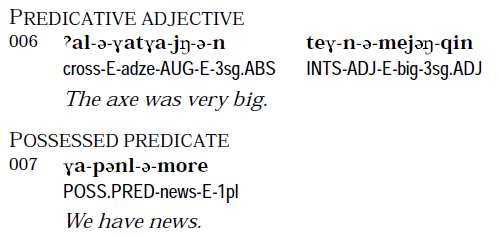
\includegraphics{Chukchi/src/chnc.png}
\end{center}
\subsection{종속절}
부동사가 종속절의 핵어를 이루며, 분사는 관계절의 핵어를 이루는 것으로 분석할 수도 있기는 하다. 접속 소사로 연결된 절은 종속절은 아니다.
\begin{itemize}
	\item{부동사절} 부동사는 부사성 하위절의 핵이 되며 아래와 같이 세 가지 접미사로 만들어진다. 논항들은 주절의 어떤 논항과도 필수적 공지시는 없으며 화용에 따라 결정된다. 
	\begin{itemize}
		\item \textbf{-ma}: 동시성(`-하는 동안')
		\item \textbf{-k}: 연속성(`-하고 나서')
		\item \textbf{-(i)neŋu} 귀결성(`-함으로 인해')
	\end{itemize}
	\item{분사절} 축치어의 분사는 동사에서 파생된 명사로, 때로는 동사의 결합가를 유지하지만 구어에서는 극히 드물다. 보통은 논항이나 (절대격) 수식어로 쓰인다.
\end{itemize}
\subsection{중/복문}
접속 소사로 절을 연결할 수 있다. 등위 접속과 종속 접속을 구분할 형태적 기준은 거의 없다. 접속된 절은 다른 절의 앞이나 뒤 혹은 단독으로 올 수 있으며, 접속사는 보통 접속된 절의 앞에 오고 드물게 뒤에 온다. 
\subsubsection{시제 연쇄}
동사는 인접한 절의 TAM과 동일한 값을 가지며, 문장 내에서는 단 한 번의 TAM 변경이 가능한 경향이 있다. 서사의 사건 구조에는 주로 서실법이 쓰인다. 마지막 둘은 덜 사실적인 맥락이다.
\begin{center}
\begin{tabular}{l|l}
사건 구조	&시제 연쇄\\
\hline
상태(변화) $\rightarrow$ 사건 &완료/습관 $\rightarrow$ 부정과거\\
사건 $\rightarrow$ 상태(변화) &부정과거 $\rightarrow$ 완료/습관\\
사건\textsubscript{i} $\rightarrow$ 사건\textsubscript{j} & 부정과거 $\rightarrow$ 부정과거\\
상태(변화) $\rightarrow$ 상태(변화) &완료/습관 $\rightarrow$ 완료/습관\\
상태 $\rightarrow$ 미래의 사건/상태 & 습관 $\rightarrow$ 미래\\
미래의 사건/상태 $\rightarrow$ 미래의 사건/상태 & 미래 $\rightarrow$ 미래\\
\hline
\end{tabular}
\end{center}
\subsubsection{문장 간 및 문장 내 등위 접속}
가장 흔한 절/술어 접속 소사는 \textbf{ənkˀam}과 \textbf{cama} `그리고'이다(전자는 명사류 접속에도 자유롭게 쓰인다) 다른 접속 소사는 의미적으로 종속 관계를 표시한다. 종류로는 \textbf{qeluq} `왜냐하면', \textbf{wətku} `-할 때만', \textbf{ecɣi} `-하자마자', \textbf{ewət/ewər} `마찬가지로'가 있다.
\subsection{양태 유형}
동사 굴절은 TAM 범주에 따라 서실법(평서 미래/비미래, 습관/보편, 완료)과 비서실법(명령/의도, 조건) 의미를 표시한다. 부정 극성, 의문, 부정 명령과 같이 통사적으로 표시되는 통사적으로 표현되는 양태도 있다. 축치 담화에는 (직접)인용 발화가 많은데, 가상의 타자로서 말하는 화용이 문법적인 여러 차이를 불러온다. 
\subsubsection{극성}
부정 극성 절은 동사에 표시되는 문법범주가 긍정보다 더 적고 명사류 논항 표시 방식도 다르다. 부정 동사는 부정 소사나 부정 동사 어기로 표시될 수 있고, TAM은 표시되는 경우 조동사를 빌린다. 부정 소사와 의도법 굴절 동사로 이루어지는 부정 절의 경우 서법 변별이 없어지고 소사의 종류를 통해 시제를 표현한다.
\subsubsection{의문}
판정 의문문에는 긍정/부정 소사나 술부의 일부를 반복하는 것으로 답변할 수 있다. 부정 질문은 답변자가 부정 명제의 진리치에 동의하는 경우 부정 답변을 해야 하고(영어식), 긍정 답변은 대안 명제를 함께 제시해야 한다. 설명 의문문 중 동사적 답변을 요구하는 것은 의문 대명사 혹은 어간 \textbf{req-} `무엇을/무언가를 하다'(자동사)나 사동형 \textbf{rəreqew-/-nreqew-}(타동사)로 만든다. 이 어간들은 부정[不定] 대동사로로도 쓰이며, 답변 시에는 타동성을 맞춰줘야 한다.
\subsubsection{명령}
의도법 범주의 주 기능으로 명령/권고적 의미가 있다. 의도법은 인칭/수 표시 패러다임이 완전하며 그 중 2인칭만이 기본적으로 명령법이다. 3인칭 의도법은 권고법적 의미를 가질 수 있으나, 1인칭의 경우 미래/희구법적 의미를 표시하는 데 쓰인다. 의문 소사와 의문/권고 억양 그리고 부정 절로 구성된 부정 판정 의문문은 약한(정중한) 명령의 효과를 가질 수 있다(`Why don't you --?').
\subsubsection{직접 및 간접 화법}
축치어에는 간접 발화를 표시할 방법이 없지만, 직접 인용 발화는 비인용 발화와 문법적 차이를 보인다.
\begin{itemize}
	\item 상상 속 타자의 발화는 억양, 음색, 성별 방언 등으로 표시된다.
	\item 화자와 때로는 청자 논항이 \textbf{iw-} `말하다' 동사에 공지시될 수 있다.
	\item 비인용 발화에서는 명시적 인칭 대명사가 대조적 기능이나 특정 통사 구문에서만 쓰이나, 인용 발화에서는 가상의 화자와 청자를 확인할 필요 때문에 많이 사용된다.
	\item 또한 대화에서는 TAM 범주가 가능한 것보다 단순하게 나타나며 비굴절 동사 어기를 사용하는 경향이 보인다.
\end{itemize}

\section{명사류 굴절}
명사류는 논항으로 쓰일 수 있는 단어들로, 격/수/인칭에 따라 굴절한다. 명사류에는 명사, 인칭/부정[不定]/지시/양화 대명사, 분사가 속한다. 명사류는 의미적으로 보통과 고등 생물이라는 생물성 부류로 나누어지며, 이 문법서에서는 전자를 원형으로 본다.
\subsection{명사류의 하위 분류}
\begin{itemize}
	\item{명사} 명사류의 주 하위 부류로서 명사류의 특징을 모두 갖는다.
	\item{인칭 대명사} 어간에 인칭/수가 내재되어 있으므로 명사에 붙는 인칭/수 접미사가 붙지 않는다. 파생 가능성이 많으며, 소유주를 포합할 수 있고 지소/확대 접사로 파생될 수 있다.
	\item{부정 대명사} 생물성 변별을 보이는 두 개의 어간 \textbf{req-} '무엇/무언가'와 \textbf{mik-} '누구/누군가'가 속한다. 전자는 보통명사, 후자는 고등 생물 명사처럼 곡용한다.
	\item{지시 대명사} 지시 대상의 생물성에 따라 고등 생물 혹은 보통 명사처럼 곡용할 수 있다. 거리에 따라 \textbf{ŋot.qen(a)-} '이것', \textbf{ŋan.qen(a)-} '저것', \textbf{ŋaan.qen(a-)/ŋoon.qen(a-)} '저어것(?)'으로 차등된다. \textbf{ən.qen(a)-}'그것'은 3인칭 단수 인칭 대명사와 동일한 어간 \textbf{ən-}을 가지며, 다른 지시사와 달리 거리가 아닌 대용적 지시 기능을 한다.
	\item{양화 대명사} \textbf{əməlˀo} `모두’와 \textbf{qut-} `하나/나머지 하나'(불규칙 절대격 단수 \textbf{qol})가 속한다. 전자는 내재적으로 복수이며 복수 일치를 받을 수 있으나 복수 접사가 붙지는 않는다.
	\item{분사} 동사 어근처럼 논항을 지배할 수 있어 다른 파생된 명사들과 통사적으로 다르다. 다음의 네 가지 구조 유형이 있다.
	\begin{center}
	\begin{tabular}{lll}
	자동 &자동 능동(S 초점) &\textbf{təle-lˀ-ə-n} `가는 이' (<\textbf{təle-} `가다')\\
	타동 &수동(O 초점) &\textbf{təm-jo} `죽임당한 이' (<\textbf{təm-/-nm-} `죽이다')\\
		&부정 수동(부정 O 초점) &\textbf{e-nm-ə-kə-lˀ-ə-n} `죽임당하지 않은 이'\\
		&타동 능동(역수동화된 A 초점) &\textbf{ine-nm-ə-lˀ-ə-n} `죽이는 이'\\
	\end{tabular}
	\end{center}
\end{itemize}
\subsection{굴절 범주: 격, 수, 인칭}
\begin{itemize}
	\item (포합/합성되지 않은) 명사류 핵어는 격/수/인칭에 따라 굴절하나 보통 절대격에서만 그러하다. 축치어의 문법격에는 절대격(S/O), 능격(A), 등격(계사 보어)이 있다. 능격은 사실 (도)구격의 기능도 가지며, 등격은 비핵심 기능 '-로서'도 수행한다.
	\item 처격 \textbf{-k}은 최소한의 공간 관계를 표시하며 부정사와 연속성 부동사 표지와 동음 관계이다. 축치어 명사류 형태론은 파생 접사로 인해 더 복잡해지는데, 예컨대 공간 관계는 격표지(\textbf{-jiŋkə} `-- 아래에'), 격표지+파생 접사(처격+\textbf{-tkən-\textsuperscript{+VH}} `-- 위에'), 후치사(\textbf{qaca} `-- 옆에') 등으로 표현할 수 있다.
	\item 격으로 분류하는 기준은 형태적으로 절대격/능격과 상보적 분포를 이루는지와 통사적으로 동사의 논항이나 부가어로 기능하는 독립 명사류를 표시할 수 있는지이다. 이에 따르면 축치어에는 총 13개의 격이 존재하며, 이는 Skorik의 분석에 4개가 추가된 것이다.
	\item 수 범주는 보통명사는 절대격에서만 표시되며 고등 생물 명사에서는 등격에서만 표시되지 않는다. 인칭 대명사를 제외한 나머지 명사류는 절대격에서 단/복수로 표시될 수 있고, 일부 명사는 개별적 수가 존재해 개별-불특정-복수의 3항 대립을 이룬다. 격 형태는 규칙적이며 아래 표와 같다. 주석 생략.
\end{itemize}
\begin{center}
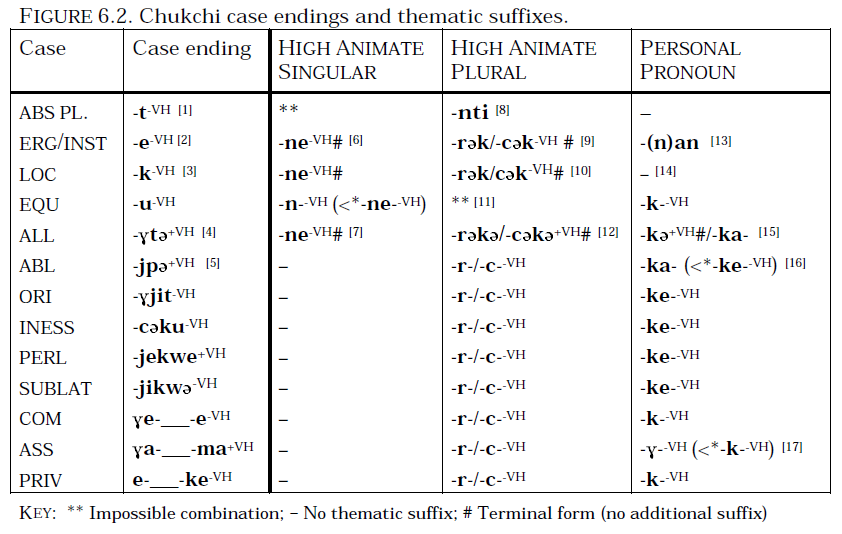
\includegraphics[width=\linewidth]{Chukchi/src/chca.png}
\end{center}
\begin{itemize}
	\item{고등 생물 명사} 인명(사람, 애완동물, 일부 정령이나 신화적 인물의 고유한 이름)과 친족 호칭어 혹은 이들을 지칭하는 지시/양화 대명사를 포함한다. 이들은 능/구격, 처격, 향격 단수형에 단일 접미사 \textbf{-ne\textsuperscript{-VH}}를 사용하며, 등격은 이 접미사에 등격 접미사를 붙인 형태이다. 인명의 복수는 해당 인물과 그가 이끄는 집단을 함께 지칭한다. 고등 생물 명사의 복수형은 어간 접미사 \textbf{-r/c-\textsuperscript{-VH}}로 표시된다. 능격은 처격과 동일한 형태인 \textbf{-rək/cək\#\textsuperscript{-VH}}, 향격은 \textbf{-rəkə/cəkə\textsuperscript{-VH}} 불규칙형을 각각 갖는다.
	\item{인칭대명사} 대부분의 경우 보통명사와 동일하게 굴절하나 어간 접미사 \textbf{-ke-}가 붙는다. 처격에서는 일반 명사처럼 굴절하며 절대격과 능/구격에서는 불규칙형이 나타난다.
\end{itemize}
\subsection{핵심적 격}
\subsubsection{절대격 단수}
명사의 절대격 단수형은 음운적 형태나 형태적 기원에 따라 여러 패턴으로 형성된다. 단모음 단음절로는 실현될 수 없다는 제약이 있다.
\begin{itemize}
	\item{Ia) 비굴절 어간} 대부분 자음으로 끝나며, 일부 명사나 수동분사 \textbf{-jo} 등은 모음으로 끝난다.
	\item{Ib) 비굴절 어간, 어말 모음 약화} e$\sim$a로 끝나는 어간에만 나타나는 유형이다. 축치어에서 이러한 모음 약화는 상당히 규칙적인 현상이다. 어말 개음절에 존재하던 성문음화도 같이 사라진다.
	\item{Ic) 비굴절 어간, 어말 모음 탈락} 탈락하는 모음에 제약은 없으며, *CCV\# 연쇄는 탈락 후 슈와 삽입이 일어난다. 합성명사의 어말 핵어는 원래 다른 유형이었더라도 종종 이 유형에 속하며, 어말 위치에서 끝 모음을 탈락시키는 명사화 접미사도 많다.
	\item{IIa) 완전 중첩} (C)VC 어간에 적용되며, 절대격 단수(보통 절대격 복수도)에서 나타난다. 다른 격이나 포합 형태는 비중첩 어간을 사용한다. IV형 단어인 \textbf{jara-ŋə} `집'과 \textbf{joro-ŋə} `침실'도 원래는 중첩형이었으나 r의 반복 출현이 이화된 형태이다.
	\item{IIb) 부분 중첩} 기저에서 2음절인 어간이 가능하다. 어말 성문음화는 모음 앞 성문 폐쇄음으로 실현되며, 제약으로 인해 /kmˀ/ $\rightarrow$ kəmˀə와 같이 슈와 삽입이 일어난다. 표면형의 첫 (C)VC 연쇄가 맨 마지막으로 중첩된다. 이때 어두 C가 없지 않은 한 성문 폐쇄음은 중첩된 음절에 옮겨가지 않는다.
	\item{III) 접미사 \textbf{-n\textsuperscript{-VH}}} 파생된 명사류에서 가장 흔한 부류이며, 비종결 접미사로 파생된 명사에는 항상 적용된다. 물론 비파생 명사들도 속한다.
	\item{IV) 접미사 \textbf{-ŋə\textsuperscript{-VH}}} 집, 침실, 솥, 접시, 순록, 망치, 바늘, 국물 등의 일부 고빈도 명사((C)VCV- 어간)가 속한다.
	\item{V) 불규칙 절대격 단수형} 매우 드물며, 일부는 자잘한 음운 변동이나 방언 혼합의 결과로 보인다.
\end{itemize}
\subsubsection{명사류 파생 접미사의 절대격 형태}
일부 명사류 파생 접미사는 파생된 명사의 형태적 부류를 결정한다. 예컨대 지소사 \textbf{-qej\#/-qej-\textsuperscript{-VH}}는 1a, 도구 접미사 \textbf{-neŋ\#/-neŋe-\textsuperscript{-VH}}는 Ic, \textbf{-tkən-ə-n\#/-tkən-\textsuperscript{-VH}} `-- 위'는 III, 동사에서 장소 명사를 파생시키는 \textbf{-n\#/-nwə-\textsuperscript{+VH}}는 V인 식이다. Ib형은 문증되지 않으며 IIa-b와 IV형은 파생법과 양립 불가능하다.
\subsubsection{개별형}
`개별적' 수 범주는 기본적으로 개별화되어 있지 않은 의미의 절대격 명사, 예컨대 한 쌍씩 있는 신체 부위/의복/물건, 열매/곡식, 작은 새/동물, 집단적으로 나타나는 별 등의 물체, 줄/끈 등에만 표시된다. 개별화 접미사의 기저형은 \textbf{*-lŋ\textsuperscript{+VH}ə-n\textsuperscript{-VH}}이며, \textbf{*-lŋ\textsuperscript{+VH}}은 모음-(기저)설정음 연쇄 앞에서 \textbf{-ləŋ-}, 나머지 경우 \textbf{-lɣ-}로 실현된다. 또한 \#CVC(C) 형식의 신체 부위 어간에만 나타나는 \textbf{-tləŋ-} 형태도 있다.
\subsubsection{절대격 복수}
모든 보통명사는 절대격 복수형이 있고, 단/복수로만 쓰이는 명사나 불규칙 복수형은 없다. 절대격 복수는 보통 \textbf{-t\textsuperscript{-VH}}로 만들지만, 설정음(t, r, c, j, n) 뒤에서 이형태 \textbf{-ti\textsuperscript{-VH}}가 나타날 수 있고 그 조건은 어휘적이다. 고등 생물 명사의 경우 어간 접미사 \textbf{*-r\textsuperscript{-VH}}와 \textbf{-ti}가 결합하여 \textbf{-n-ti}로 실현된다. 인명의 복수형은 그 사람과 그의 가정을 통칭한다. 아버지와 어머니 둘 다 복수형(\textbf{ətləɣ-ə-t/ətlˀa-t})에서 부모를 의미할 수 있고, 한쪽 성별인을 지칭하는 다른 명사도 비슷한 행동을 보인다. 
\subsubsection{능격/구격}
\begin{itemize}
	\item 능격과 구격은 형태적으로 동일하나 통사적으로 다른 기능을 한다. 구격은 `도구/수단' 의미역을 주로 표시하며, 이 때문에 구격을 받는 명사류는 흔히 무생물이다. 축치어에서는 생략이 빈번하여 능격과 구격이 한 문장에서 잘 나오지는 않지만 도출은 쉽다. 아래와 같은 예시가 문증된다.
\begin{center}
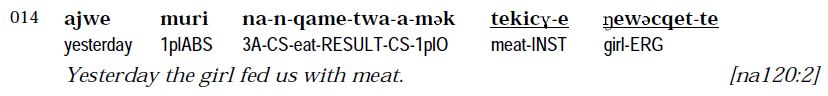
\includegraphics[width=\linewidth]{Chukchi/src/chei.png}
\end{center}
	\item 어떤 자동사의 어휘적 사격 논항들은 구격으로 표시되며, \textbf{qame-} `먹다' 등 섭취 동사의 사격 목적어(먹히는 것)는 규칙적으로 구격으로 표시된다. Skorik에 따르면 역수동화된 동사의 사격 논항이 구격으로 표시된다고 하나 확인되지 않았다.
	\item 동사 어기를 형성하는 접미사 중 하나가 형태적으로 능/구격과 동일하다.
\end{itemize}
\subsubsection{등격}
\begin{itemize}
	\item 등격은 계사 보어 기능과 비계사절에서 유사한 기능을 하는 사격 명사류를 표시하는 기능을 한다.
	\item 등격은 항상 수가 표시되지 않는다.
	\item 영계사 구문에서는 보어가 등격이거나 절대격이며, 계사가 있는 경우 등격 표시는 필수이다.
	\item 사격 기능에서 부수적 술어의 핵어로 선택되는 논항은 S/O이다.
	\item \textbf{-ne} 어간 접미사로 형성되어 \textbf{-nu}로 실현되는 고등 생물 곡용형이 존재한다.
\end{itemize}
\subsection{장소적 격}
축치어는 다양한 공간 관계를 명사류에 격 접미사나 파생 접미사 혹은 부사 접어로 표시한다. 내격 접미사는 방향격과 결합될 수 있다는 점에서 파생성을 띤다. 
\begin{itemize}
	\item 기본 공간격은 세밀한 의미가 없는 처격 \textbf{-k\textsuperscript{-VH}}이다.
	\item 방향격은 대상 쪽으로 가는 움직임을 나타내는 향격 \textbf{-ɣtə\textsuperscript{+VH}}, 대상이나 구내에서 멀어지는 움직임을 나타내는 탈격 \textbf{-jpə\textsuperscript{+VH}}, 경로를 따라가는 움직임을 나타내는 통격 \textbf{jekwe\textsuperscript{+VH}}이 있다.
	\item 종격은 지시 지점이 되는 대상을 표시하나, 본질적 방향성은 없다.
	\item 이동을 특정하지 않고 위치를 표시하는 격으로는 대상 안에 위치함을 나타내는 내격 \textbf{cəku\textsuperscript{-VH}}과 대상 아래에 위치함을 나타내는 하격 \textbf{jiŋkə\textsuperscript{-VH}}이 있다.
\end{itemize}
\subsection{수반적 격}
모든 수반적 격은 동사 어기와 동음어 관계이다. 격에 더해 사람이 사람을 수반함을 나타내는 후치사 \textbf{reen}도 있다.
\subsubsection{공동격}
공동격은 다른 명사류를 수반하는 명사류에 표시되며, 두 논항은 보통 위계가 동등하다. 출현은 비교적 드물며 아래의 참여격이 훨씬 흔하다. 표지는 접환사로서 다음과 같은 이형태 분포를 보인다.
\begin{center}
\begin{tabular}{ll}
\textbf{ɣe-$\rule{1cm}{0.2mm}$-te\textsuperscript{-VH}} &동사로 끝나는 어간\\
\textbf{ɣe-$\rule{1cm}{0.2mm}$-e\textsuperscript{-VH}} &나머지\\
\end{tabular}
\end{center}
\subsubsection{참여격}
참여격은 핵어의 일부 혹은 소유인 무언가가 수반됨(`사람들이 무리와 함께', `집들이 거주자와 함께', `동물 가죽이 그 다리와 함께', `솥이 (내용물)과 함께' 등)을 표시하며, 표지는 \textbf{ɣa-$\rule{1cm}{0.2mm}$-ma\textsuperscript{+VH}}이다.
\subsubsection{결여격}
결여격은 무언가의 부재나 부족을 나타내는 격으로, 보통 불변화사 \textbf{ujŋe} `아니다, 없다'와 함께 쓰인다.